\section{Introduction}
\label{section:s_introduction}

\subsection{What is SpyGlass?}
SpyGlass is, generally speaking, an application to visualize sensor networks on a screen. Thereby, SpyGlass is not only able to display
some nodes at their location on a map, but can show particular data, relationships between nodes or statistical data as well.
The whole range of opportunities will be explained in this document.

SpyGlass bases on the requests given by the ITM of the University Lübeck and was developed by Daniel Bimschas, Sebastian Ebers,
Dariush Forouher and Oliver Kleine in the context of a case study for professional product development.

\subsection{Installation}

\paragraph{Prerequisites}

To run Spyglass at least JRE 6.0 is necessary. Supported platforms are

\begin{itemize}
  \item{Linux x86}
  \item{Linux AMD64}
  \item{Windows (32bit)}
  \item{Darwin 64bit}
\end{itemize}

\paragraph{Install instructions}

Spyglass can be used in two ways:

\begin{itemize}
  \item{Either as a standalone application or}
  \item{as a plugin inside the iShell tool.}
\end{itemize}

Since Spyglass uses the SWT framework, one has to
decide at compile-time which platform one wants to use.

Building Spyglass is very easy. One does not need any external
libraries besides a working Java SDK and "ant".
The resulting jar files contain all needed libraries (via the
"one-jar" boot-mechanism) and are directly executable.


\paragraph{Building Spyglass as a standalone application}

Just run one of

\begin{verbatim}
    $ ant standalone-linux
    $ ant standalone-linux64
    $ ant standalone-win32
    $ ant standalone-osx
\end{verbatim}

depending on the platform you want to run Spyglass on.

These commands will build the file ``spyglass-XXX-standalone.jar''.
This jar file includes all necessary dependencies and can be run directly via

\begin{verbatim}
    $ java -jar spyglass-XXX-standalone.jar
\end{verbatim}

\paragraph{Building iShell with Spyglass included as a plugin}

To build iShell with SpyGlass plugin one needs to run one of the commands

\begin{verbatim}
    $ ant ishell-linux
    $ ant ishell-linux64
    $ ant ishell-win32
    $ ant ishell-osx
\end{verbatim}

depending on the platform one wants to use.

These commands will build the file ``ishell-XXX-spyglass.jar''.
This jar files includes a version of iShell, the compiled Spyglass source
and all libraries both applications depend on.

Similary, it can be run directly via

\begin{verbatim}
    $ java -jar ishell-XXX-spyglass.jar
\end{verbatim}

Thats it.

\subsection{The Appearance of the application}

As mentioned before, there are two different ways to start SpyGlass. First one can start the standalone application,
secondly it is a plugin for
iShell. So one must start iShell first and activate the SpyGlass plugin afterwards.
There are some differences in the functionality of both standalone and iShell plugin but this will be discussed later.
Almost all screenshots included in this manual are from SpyGlass as an iShell plugin. This does not have a particular reason
but consistency.

On the first start of SpyGlass with an empty configuration one can just see some buttons and a large white area as one
can see in figure \ref{pic:spyglass_first_appearance}.
The standalone application has a menu bar in addition, whose entries provide the same functionality as the buttons. The white
area is called drawing area, since all visualisation of the network will take place here.

\begin{figure}[htb]
  \begin{center}
    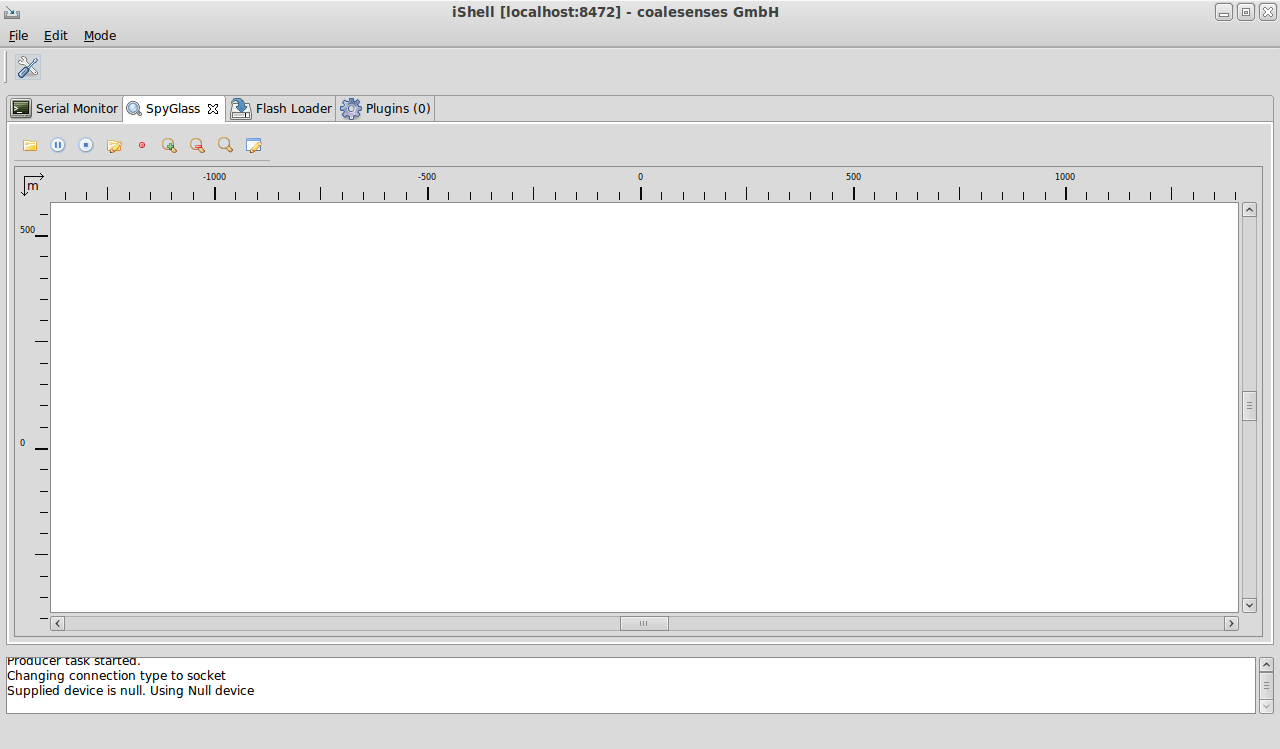
\includegraphics[width=13.2cm]{./pics/spyglass_first_appearance}
    \caption{Empty screen of the SpyGlass plugin for iShell}
    \label{pic:spyglass_first_appearance}
  \end{center}
\end{figure}

On the bottom of the iShell window a second area appears where iShell prints out several messages during the
running time of the application.

\subsection{Buttons and their behaviour}

\begin{figure}[htb]
  \begin{center}
    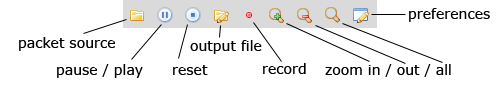
\includegraphics[width=5cm]{./pics/spyglass_buttons}
    \caption{SpyGlass buttons}
    \label{pic:spyglass_buttons}
  \end{center}
\end{figure}

The buttons located on top of the window provide some functions concerning
\begin{itemize}
  \item{the source of information, e.g the packet source,}
  \item{the zoom level and}
  \item{at least all other preferences}.
\end{itemize}

\paragraph{Packet source}

The most left button with the folder opens a dialog to define the current packet source. The source can either be iShell or
a file. For the standalone application it is only possible to chose a file as packet source. How such a packet source file
can be generated is explained later in this chapter. If the packet source is iShell, then the packets come from network.
The real packet source then must be configured by setting the TCP/IP preferences of iShell.

To explain the functionality of the pause button one must anticipate the usage of packets and plugin instances. Packets
coming from the packet source (either a network or a file) will be delivered to plugin instances. These instances
handle the packets, e.g. extract specific information and compute this information. It is not important to understand
this completely right now. Anyway, the pause button stops the packet delivery to the plugin instances and thus
freezes the current information of all plugins. That does not mean necessarily, that the illustration on the drawing area
freezes as well. Some objects on the drawing area could disappear because they time out or they could move to another
position for any reason.

All new packets coming during the time, when SpyGlass is paused are queued. They are delivered sequentially after the
play button has been clicked. The pause button changes to a play button automatically when the pause button was clicked
and vice versa.

The reset button holds the configuration but throws all past packet information away, i.e. all past packets are ignored from
now on.

The record button is to start the recording of incoming packets. One must specify a file, where the incoming packets will be
written into. The file gets the ending ``.rec'' and can be used later in both the standalone application and the
SpyGlass iShell plugin as a packet source. The record stops if one clicks on the record button again. During the recording
time, the button is white. Otherwise it is red.

\paragraph{Zoom}

The ``+'' and ``-'' buttons with the magnifier are pretty self-explanatory. One zooms in (+) while the other zooms out (-).
The third magnifier button zooms exactly to the zoom level that all current network components (nodes) are displayed on the
drawing area.

\paragraph{Open preferences}

This last button opens the preferences dialog, that is described in detail from chapter \ref{section:plugins} on.


\subsection{Drawing area and ruler}

As already explained, the drawing area shows a sector of the whole network. This sector can be enlarged by zooming out
or downsized by zooming in. To change the sector to be shown on the drawing area without changing the zoom level,
one can either use the scrollbars
on the bottom and on the right side of the drawing area or hold the left mouse-button when the pointer is located on the
drawing area and move the mouse to the desired direction.

Additionally to the buttons zooming can also be done with the scroll-wheel on the mouse, if the pointer is located
on the drawing area.

The ruler is located on the top and on the left side of the drawing area. Its labeling represents the current sector
of the drawing area with respect to the real coordinates. Thus the labels of the ruler change automatically,
whenever the drawing area is either moved or if the zoom level changes.